\documentclass[12pt]{article}
\def\activityid{F05-K-v2}\usepackage[letterpaper,margin=.65in,top=.60in,bottom=.65in]{geometry}
\usepackage[T1]{fontenc}\usepackage[default]{sourcesanspro}
\usepackage{microtype,tikz,array,tabularx,fancyhdr,amsmath}\usepackage[hidelinks]{hyperref}
\usetikzlibrary{arrows.meta,calc}
\setlength{\parindent}{0pt}\setlength{\parskip}{7pt}\setlength{\headheight}{0pt}\setlength{\footskip}{26pt}\setlength{\emergencystretch}{2em}
\pagestyle{fancy}\fancyhf{}\renewcommand{\headrulewidth}{0pt}\renewcommand{\footrulewidth}{.4pt}
\fancyfoot[L]{\scriptsize Bellingham Math Circle / Week 5 / \activityid}\fancyfoot[R]{\scriptsize \thepage}
\definecolor{ink}{gray}{.12}\definecolor{soft}{gray}{.95}\color{ink}
\newcommand{\PageTitle}[2]{{\fontsize{10}{12}\selectfont\bfseries WEEK 5\quad TOWER LAB\hfill #1\par}\vspace{3pt}{\fontsize{26}{29}\selectfont\bfseries #2\par}\vspace{2pt}}
\newcommand{\NameLine}{{\small Name: \rule{2.65in}{.4pt}\hfill Date: \rule{1.35in}{.4pt}\par}\vspace{4pt}}
\newcommand{\Task}[2]{\par\vspace{3pt}{\large\bfseries #1}\par #2\par}
\newcommand{\Subhead}[1]{\par\vspace{3pt}{\large\bfseries #1}\par}
\newcommand{\RuleBox}[1]{\par\begingroup\setlength{\fboxsep}{8pt}\colorbox{soft}{\parbox{\dimexpr\linewidth-16pt\relax}{#1}}\endgroup\par}
\newcommand{\WriteBox}[2]{\par\textbf{#1}\par\vspace{2pt}\begin{tikzpicture}\draw[black!40,line width=.5pt] (0,0) rectangle (\dimexpr\linewidth-.5pt\relax,#2);\end{tikzpicture}\par}
\newcommand{\StudentFooter}{\vfill{\small Build first. Explain by pointing, talking, or drawing.}\par}
\newcommand{\Code}[1]{\texttt{#1}}

\hypersetup{pdftitle={Week 5: k-1}}
\begin{document}
\PageTitle{K--1}{What can the tiny person see?}\NameLine
\RuleBox{Build towers of heights 1, 2, and 3. Taller towers hide shorter towers behind them. Look from one end. Count \textbf{towers you can see}, not cubes.}
\Task{1. Build and look.}{Play with your towers. Then copy this row and look from both ends.}\begin{center}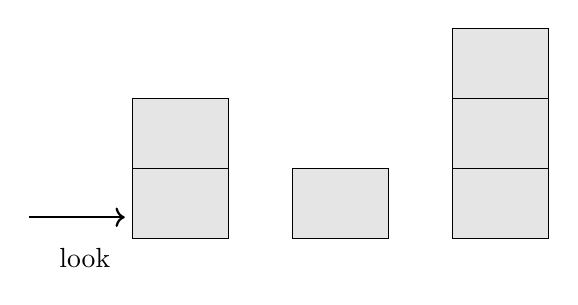
\begin{tikzpicture}[x=.8in,y=.35in]\foreach \x/\h in {0/2,1/1,2/3}{\draw[fill=black!10](\x,0)rectangle(\x+.6,\h);\foreach \j in {1,...,\h}{\draw(\x,\j)--(\x+.6,\j);}}\draw[->,thick](-.65,.3)--(-.05,.3);\node[below]at(-.3,0){look};\end{tikzpicture}\end{center}
\Task{2. Same towers, different views.}{Make a row showing all three towers from the left. Now make a row showing just one. Can you show exactly two?}
\WriteBox{Draw a row with two visible towers. Circle the towers you see.}{1.4in}
\Task{3. Two ends at once.}{Can you make a row that shows two towers from the left \textbf{and} two from the right? Can it show one from each end? Try; then explain.}
\StudentFooter
\newpage
\PageTitle{K--1}{Have we found every skyline?}\NameLine
\Task{4. Find all the orders.}{Move the towers. Have an adult record each new order. Keep the left end fixed: turning the row around may make a new order.}\begin{center}\renewcommand{\arraystretch}{2.2}\begin{tabular}{c|p{2in}|c|c} &Tower order&Seen left&Seen right\\\hline 1&&&\\2&&&\\3&&&\\4&&&\\5&&&\\6&&&\end{tabular}\end{center}
\WriteBox{How can we be sure no order is missing?}{.7in}
\Task{5. A tiny city.}{Use heights 1 and 2 once in \textbf{every row and every column}. Find both cities. Which one shows two towers from the left of the top row?}\begin{center}\begin{minipage}{.47\linewidth}\centering 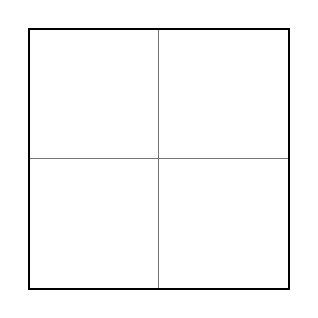
\begin{tikzpicture}[x=0.65in,y=0.65in]\draw[step=1,black!55] (0,0) grid (2,2);\draw[thick](0,0)rectangle(2,2);\end{tikzpicture}\end{minipage}\hfill\begin{minipage}{.47\linewidth}\centering 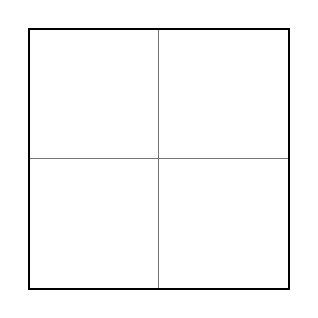
\begin{tikzpicture}[x=0.65in,y=0.65in]\draw[step=1,black!55] (0,0) grid (2,2);\draw[thick](0,0)rectangle(2,2);\end{tikzpicture}\end{minipage}\end{center}\StudentFooter
\end{document}
